\documentclass[a4paper]{article}
\usepackage[pdftex]{graphicx}
\usepackage[utf8]{inputenc}
\usepackage{enumerate}
\usepackage{siunitx}
\sisetup{locale=DE} 
\DeclareSIUnit \parsec {pc}
\DeclareSIUnit \lightyear {ly}
\DeclareSIUnit \annum {a}
\usepackage{icomma}
\usepackage{amssymb}
\usepackage{tikz}
\usepackage{href-ul}
\hypersetup{
	colorlinks=true,
	linkcolor=blue,
	urlcolor=blue}
\usepackage{geometry}
\geometry{a4paper, top=15mm, left=15mm, right=15mm, bottom=15mm,
	headsep=10mm, footskip=12mm}
\hyphenation{Bahn-ra-dius}


\begin{document}
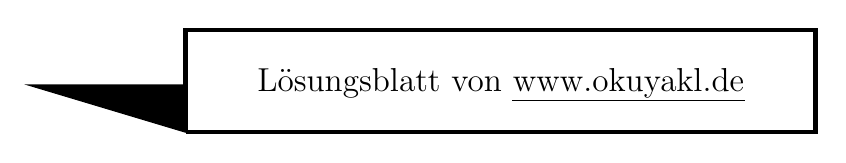
\begin{tikzpicture}(10,3)
	\draw[ultra thick](2,0) --(10,0) -- (10,1.3) --(2,1.3) -- (2,0);
	\draw[fill=black](2,0)-- (0,.6) -- (2,.6) -- (2,0);
	\node at (6,.6) {\large Lösungsblatt von \href{https://www.okuyakl.de}{www.okuyakl.de}};
\end{tikzpicture}
\vspace{0.5 cm}


\noindent {\bf Aufgabe 1. a)}\\
Es wird eine Kreisbewegung angenommen:
$$ v = \omega \cdot r = \left( {2 \pi \over T } \right) \cdot r = \left( {2 \pi \over 5,88 \cdot 24 \cdot \SI{3600}{\second}} \right) \cdot \SI{354e6}{\meter}  = \SI{4,38}{\kilo\meter}$$
\vspace{0.5 cm}

\noindent {\bf Aufgabe 1. b)}\\
Nach dem 3. Kepler'schen Gesetz errechnet sich mit den Bahndaten des Mondes Triton und mit ${T_1^2 \over T_2^2} ={a_1^3 \over a_2^3}$:
$$ a_1 = \sqrt[3]{360,1^2 \over 5,88^2} \cdot 354 \cdot 10^6 =\SI{5,5e9}{\meter} $$ 
\vspace{0.5 cm}

\noindent {\bf Aufgabe 2.}\\
Die Erdbahn ist eine Ellipse. Das zweite Kepler'sche Gesetz besagt, dass der Fahrstrahl von der Sonne zur Erde in gleichen Zeitabschnitten gleich große Flächen überstreicht, das bedeutet, dass die Bahngeschwindigkeit der Erde in sonnennahen Punkten schneller ist als in sonnenfernen. Der sonnennächste Punkt, das Perihel, wird am 6. Januar erreicht, während der sonnenfernste Punkt, das Aphel, im Juli durchlaufen wird. Die Erde bewegt sich somit etwas langsamer durch das Sommerhalbjahr als durch das Winterhalbjahr.
 \vspace{0.5 cm}
 
\noindent {\bf Aufgabe 3.}
\begin{itemize}
    \item $\SI{3}{\kelvin}$-Hintergrundstrahlung: Sie ist ein möglicher Überrest, ein Nachhall sozusagen     des ,,Big Bang's"
    \item  Die Rotverschiebung entfernter Galaxien: Daraus folgt, dass das Universum expandiert, ähnlich wie nach einer Explosion
    \item Das Vorherrschen des Wasserstoffs unter den Elementen. Im Laufe der Zeit werden in Sternen schwerere Elemente fusioniert. Dies bedeutet, dass das Universum ein begrenztes Alter hat.
\end{itemize}
\vspace{0.5 cm}

\noindent {\bf Aufgabe 4.}\\
$$ d={v_g \over H_0}= {\SI{331}{\kilo\meter\over \second}  \over \SI{74}{\kilo\meter\over \second\cdot\mega\parsec}} =\SI{4,47}{\mega\parsec}$$ 
\vspace{0.5 cm}

\noindent {\bf Aufgabe 5. a)}\\
Zunächst rechnen wir ein Lichtjahr in Kilometern aus:
$$ \SI{1}{\lightyear} = c \cdot t = \SI{2,997e5}{\kilo\meter\over \second} \cdot 365 \cdot 24 \cdot \SI{3600}{\second} = \SI{9,5e12}{\kilo\meter}$$
Die Entfernung des Nebels ist also (in km):
$$3,0 \cdot 10^6 \cdot \SI{9,5e12}{\kilo\meter} =\SI{2,9e19}{\kilo\meter}$$
Der Zeitpunkt des Zusammentreffens ist T:
$$ T = {s \over v }= {\SI{2,9e19}{\kilo\meter}\over \SI{190}{\kilo\meter\over \second} } = \SI{1,5e17}{\second} = \SI{4,7e9}{\annum} $$  
\vspace{0.5 cm}

\noindent {\bf Aufgabe 5. b)}\\
Auf nahe Objekte wirkt die Gravitationskraft. Nur sehr weit entfernte Objekte werden mit der Expansion des Universums fortgetragen.
\vspace{0.5 cm}

\noindent {\bf Aufgabe 6.}\\
\includegraphics[width=9 cm]{milchstraL123}
\vspace{0.5 cm}

\noindent {\bf Aufgabe 7. a)}\\
Planeten bewegen sich auf Ellipsenbahnen um die Sonne, die in einem der beiden Brennpunkte steht.
\vspace{0.5 cm}

\noindent {\bf Aufgabe 7. b)}\\
Die Sonne bewegt sich zusammen mit ihrem Planetensystem um das Zentrum der Galaxis.
\vspace{0.5 cm}

\noindent {\bf Aufgabe 7. c)}\\
In gleichen Zeitabschnitten überstreicht der Fahrstrahl zwischen Sonne und Planet gleiche Flächen.
\vspace{0.5 cm}

\noindent {\bf Aufgabe 7. d)}\\
Befindet sich die Erde im Aphel ihrer Bahn, dann hat sie den größten Abstand zur Sonne.
\vspace{0.5 cm}

\noindent {\bf Aufgabe 7. e)}\\
Hubble entdeckte eine Rotverschiebung im Spektrum der Sterne und folgerte, dass sich die Galaxien um so schneller von der Erde entfernen, je weiter sie weg sind.
\vspace{0.5 cm}

\noindent {\bf Aufgabe 7. f)}\\
18 Kilometer pro Stunde bedeuten, dass er in 10 min = ${1 \over 6}\SI{}{\hour}$, also ${18 \over 6}= \SI{3}{\kilo\meter}$
zurücklegt.
\vspace{0.5 cm}

\noindent {\bf Aufgabe 7. g)}\\
Erstens bewegt sich die Milchstraße im Universum relativ zu anderen Galaxien, und zweitens befindet sich unsere Sonne in einem seitlichen Spiralarm unserer Galaxis. 
\vspace{0.5 cm}

\begin{center}
	\includegraphics[width=7 cm]{../../viecher/endcomic.pdf}
	
	Hier geht es zurück zum \href{https://www.okuyakl.de/phys/p10astL123/aa123.pdf}{Aufgabenblatt}
\end{center}

\end{document}
